\chapter{Collecte de données}

Cette section décrit la collecte de données ouvertes permettant de calculer la variabilité du Taux de CHarge de la production solaire (TCH solaire) ainsi que de l’expliquer, de manière à permettre par la suite une modélisation robuste et basée sur des observations physiques pertinentes. On vise ainsi une prédiction de la variabilité du TCH à 30 minutes dans le futur, pour permettre aux opérateurs du réseau de prendre d’éventuelles mesures préventives sur le réseau électrique en cas de de forte variabilité.

\section{Données de production}

Des données de production d’énergie sur le territoire Français sont mises à disposition par RTE. Il est possible de télécharger ces données pour la région PACA sur le site éCO2mix (licence Etalab) : elles sont disponibles pour les années 2013 à 2025, à raison d’un jeu de données par année.

La première exploration de ces données montrent que la {\bfseries variabilité du TCH n’est pas disponible en l’état dans ces données} : il est donc nécessaire de la calculer, par exemple de la manière suivante (le détail de ce choix sera donné dans les sections suivantes) :

\begin{equation}
\left| V(t + \Delta t) \right| = \left| \frac{P(t+\Delta t) - P(t)}{P_{capacite}} \right| = \left| TCH(t + \Delta t) - TCH(t)\right| = \left| \Delta TCH(t + \Delta t) \right|
\end{equation}

Avec :
\begin{itemize}
\item $V$ : la valeur absolue de la variabilité du taux de charge de la production solaire (variable cible pour cette étude) ;
\item $P$ : la production d’énergie solaire (disponible pour toutes les années sous le nom Solaire’) ;
\item $P_{capacite}$ : la capacité du parc de production installé (varie au fil du temps, non disponible dans le jeu de données éCO2mix et complexe à reconstruire) ;
\item $TCH$ : le taux de charge de la production solaire (disponible pour les années 2020 à 2025)
\end{itemize}

L'objectif du projet sera donc de résoudre un problème de régression supervisée.

La variable idéale pour ce calcul est le TCH solaire, mais cette variable n’est disponible qu’à partir de l’année 2020. Entre 2020 et 2025, 106 704 observations sont disponibles dans éCO2mix, ce qui reste raisonnable pour cette étude : on décide donc de se limiter aux années 2020 à 2025.

Or les années 2020 à 2025 ne présentent {\bfseries pas toutes le même nombre de variables} : on commence par rechercher les variables communes puis on ne conserve dans ces variables communes que {\bfseries celles concernant la production d’énergie solaire}, ainsi que la consommation. Cette dernière variable pourrait en effet présenter un intérêt pour la modélisation car en cas de forte production mais de faible demande, les opérateurs du réseau peuvent être amenés à limiter la production d’énergie photovoltaïque, voire à la couper. Idéalement, le modèle final pourrait capter ce type de situation pour limiter la gêne occasionnée sur le réseau.

A cette étape, on conserve 6 variables : \textit{date}, \textit{heures}, \textit{consommation}, \textit{solaire}, \textit{tco\_solaire}, \textit{tch\_solaire} (le détail des variables sera donné dans la section Analyse exploratoire~\ref{subsec:var_dispo}).

Ces données ne contiennent aucun élément permettant d’expliquer la production d’énergie solaire : on sait que de nouvelles données explicatives devront être agrégées à ces premières variables collectées.

Or les variables idéales pour agréger de nouvelles données sont la date et l’heure des observations. On s’interroge alors sur le fuseau horaire utilisé par RTE : s’agit-il d’un fuseau UTC ou du fuseau horaire de France métropolitaine ? Les données explicatives fournies par RTE avec le jeu de données ne le précise pas.

On va donc observer comment varie la production d’énergie solaire entre deux dates où l’on sait qu’un changement d’heure à eu lieu en France métropolitaine. \textbf{Observe-t-on un décalage horaire dans la production} entre le jour avant et le jour suivant le changement d'heure ?

\begin{itemize}
\item Si oui : le fuseau horaire est bien celui de France métropolitaine ;
\item Sinon : le fuseau horaire est peut être le fuseau UTC.
\end{itemize}

\begin{figure}[htbp]
    \centering
    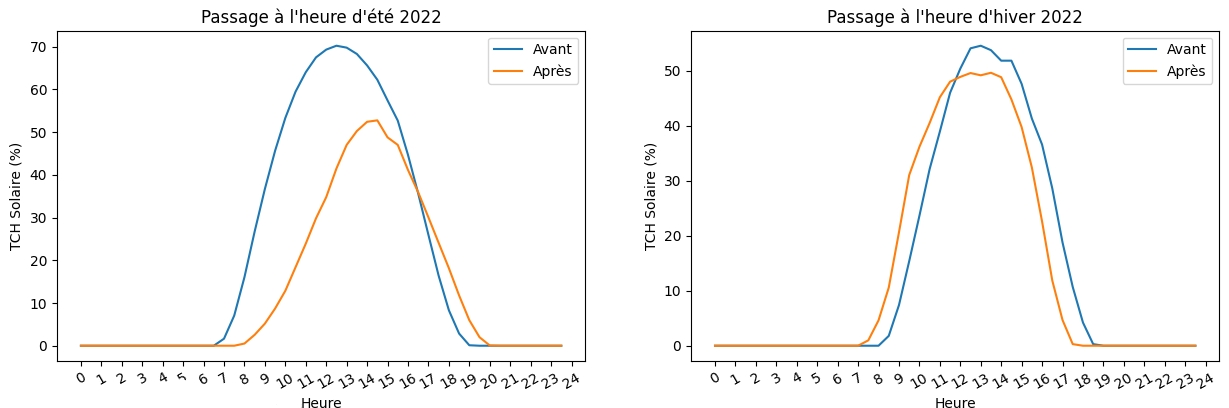
\includegraphics[width=0.8\textwidth]{img/heures_ete_hiver.jpg}
    \caption{Changements d'heure en 2022.}
    \label{fig:changement_heure}
\end{figure}

On observe bien un décalage horaire : la production est décalée une heure plus tard lors du passage à l’heure d’été et une heure plus tôt lors du passage à l’heure d’hiver.

La date et l’heure de France métropolitaine sont converties en une seule variable \textit{datetime\_utc}, de manière à pouvoir agréger de nouvelles données facilement par la suite (toutes les données suivantes seront collectées sur la base d’une heure UTC).

Pour clore cette première partie de la collecte de données, on calcule notre variable cible (valeur absolue de la variabilité du tch solaire à l’instant t + 30 minutes) : on dispose à ce stade de 106 704 observations pour 6 variables (\textit{datetime\_utc}, \textit{consommation}, \textit{solaire}, \textit{tco\_solaire}, \textit{tch\_solaire}, \textit{target}).

\begin{figure}[htbp]
    \centering
    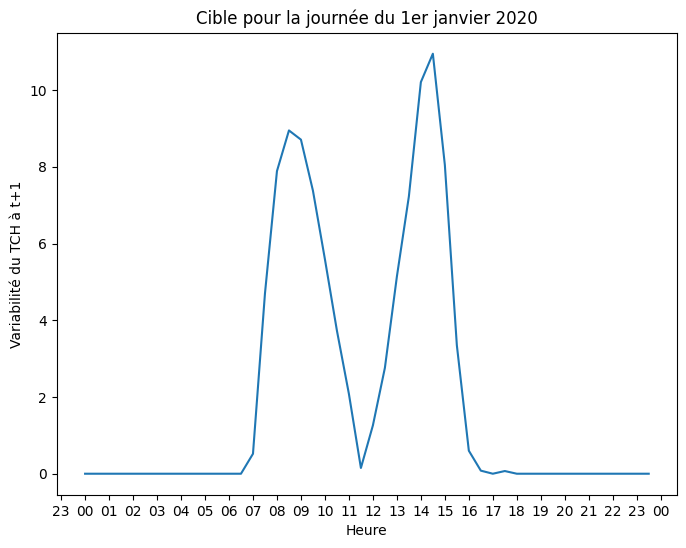
\includegraphics[height=5cm]{img/cible.png}
    \caption{Valeur absolue de la variabilité du Taux de CHarge de la production solaire (TCH).}
    \label{fig:cible}
\end{figure}

\textbf{Plus de détails} sur les opérations réalisées pour la collecte des données de production sont disponibles dans notebooks/02\_Collecte/02\_collecte\_01\_production.ipynb.

\section{Données astronomiques}

Les données de \textbf{production d'énergie solaire} sont collectées et la variable cible construite, mais les variables collectées ne permettent à priori pas d'expliquer la variable cible.

\begin{itemize}
\item Elles ne contiennent pas de données sur la \textbf{position du soleil} par rapport aux panneaux solaires ;
\item Ni de données météorologiques ;
\item Ni de données atmosphériques.
\end{itemize}

Pour déterminer quelles données pourraient permettre d'expliquer notre variable cible et pourraient être utiles à notre modélisation, on part des connaissances usuelles de l'homme du métier (voir les articles retenus dans les Annexes).

Parmi ces connaissances, on a constaté que la position du soleil par rapport à l'emplacement des panneaux solaires était importante et que cette position était déterminée par l'\textbf{azimut} et l'\textbf{angle solaire}.

On a vu que la région PACA était vaste et on a déterminé \textbf{cinq lieux significatifs} pour la production d'énergie solaire : on calcule l'azimut et l'angle solaire pour chacun d'eux, à l’aide de la librairie Python \textbf{PySolar}, librement mise à disposition par des passionnés d’astronomie, pour chaque date présente dans le jeu de données précédemment collecté.

\textbf{Plus de détails} sur les opérations réalisées pour la collecte des données astronomiques sont disponibles dans notebooks/02\_Collecte/02\_collecte\_02\_astronomie.ipynb.

\section{Données atmosphériques}

Pour l'homme du métier, d'autres données que celles concernant la position du soleil pourraient permettre d'expliquer notre variable cible et être utiles à notre modélisation. On s’intéresse dans cette section aux \textit{rayonnements solaires effectivements reçus} au niveau des panneaux solaires et donc à des données concernant l'\textbf{atmosphère}.

Ces données sont par exemple disponibles dans un jeu de données \textbf{CAMS solar radiation time-serie} mis gracieusement à disposition par Copernicus (\href{https://www.copernicus.eu/fr}{programme d’observation de la Terre de l’Union européenne}), sous licence CC BY 4.0.

Pour chacun des points d'intérêts identifiés pour la production d'énergie solaire, on collecte 4 variables concernant l’irradiance reçue au niveau des panneaux solaire (\textit{GHI}, \textit{BHI}, \textit{DHI} et \textit{BNI}) ainsi que leur 4 équivalents au sommet de l’atmosphère (\textit{valeur théorique maximale} obtenue par temps clair).

Ces variables sont collectées via une API dédiée entre la première et la dernière date de notre jeu de données, avec une \textbf{résolution temporelle de 15 minutes}. Comme les variables que nous sommes en train de collecter sont \textbf{cumulatives}, on les sommes deux à deux pour obtenir des données pour 30 minutes. On ne conserve ensuite que les observations dont la date est présente dans le jeu de données de production.

\textbf{Plus de détails} sur les opérations réalisées pour la collecte des données atmosphériques sont disponibles dans notebooks/02\_Collecte/02\_collecte\_03\_atmosphere.ipynb.

\section{Données météorologiques}

Pour terminer la collecte de données et compléter les variables explicatives, on cherche maintenant à récupérer des \textbf{informations météorologiques} complémentaires, telles que :

\begin{itemize}
\item La \textit{température} au sol (influe sur la performance des panneaux solaires) ;
\item La \textit{vitesse du vent} au sol (influe sur la performance des panneaux solaires) ;
\item L'\textit{humidité} (influe sur la performance des panneaux solaires) ;
\item La \textit{nébulosité} (influe sur la lumière reçue par les panneaux solaires).
\end{itemize}

On peut trouver ces données dans un dataset mis à disposition par la NASA via une API : \href{https://power.larc.nasa.gov/}{POWER Hourly API}, sous licence Creative Commons BY 4.0.

Cette base de données a une résolution temporelle d'une heure : comme les données précédentes ont une résolution de 30 minutes et qu’on souhaite garder cette précision pour notre variable cible, on interpole les données météorologiques.

Enfin, l’instrument de mesure de la nébulosité utilisé ici est arrivé en fin de vie le 30 décembre 2025 : les observations suivantes sont supprimées.

\textbf{Plus de détails} sur les opérations réalisées pour la collecte des données météorologiques sont disponibles dans notebooks/02\_Collecte/02\_collecte\_04\_meteorologie.ipynb.

\section{Bilan de la collecte}

Quatre jeux de données ont été collectés concernant la production d’énergie solaire, des données astronomiques, atmosphériques et météorologiques. Ces quatre jeux sont fusionnés en un seul jeu de données par un merge sur la variable \textit{datetime\_utc} commune à tous.

